\begin{figure*}[t]
\centering
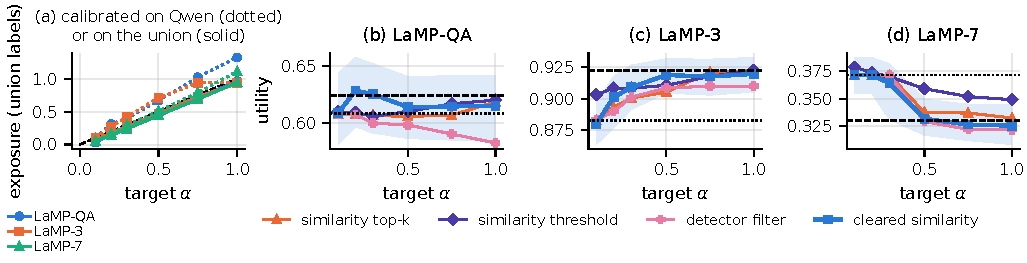
\includegraphics[width=\textwidth]{generated/fig_main.pdf}
\caption{(a) Exposure under union labels of test users, worst of four rules,
for rules calibrated on the primary auditor (dotted) or on the union
(solid). (b--d) Cross-fitted utility of the rules calibrated on union labels,
with a 95\% band for cleared similarity. Dotted is no profile, dashed top-5.}
\Description{Four panels show exposure versus the target and task utility
versus the target for four admission rules. Union calibration reduces measured
exposure; the utility cost varies across the three tasks.}
\label{fig:main}
\end{figure*}
